\chapter{Background}\label{chap:background}

\section{Soup}

\section{Rust}
\subsection{Foreign Function Interface}

\section{Recovery}

\section{bincode}

\section{Profiling}

\section{SQLite}\label{sec:sqlite}
SQLite~\cite{sqlite} is by far the most widely deployed database ever written.
Used in everything from smart phones to cars, with an estimated user count in
the magnitude of multiple billion users, SQLite is everywhere\footnote{Who
uses SQLite? \url{https://www.sqlite.org/mostdeployed.html}}. SQlite is an
embedded database, and requires no extra processes, or even threads, to run.

In a world of unreliable software, SQLite is stable as a rock. It has 100\%
branch test coverage, with a test suite containing millions of different test
cases. SQLite is, and always has been, available in the public domain. As the
name implies, SQLite provides an SQL interface to developers, with decent support
for everything from indices to views. The library itself is written in about 130
thousand lines of C code.

While the main usage of SQLite is as a persistent application store (\eg in
browsers and mobile applications), SQLite is also popularly used as an engine in
other databases. One such example is the recently open-sourced
FoundationDB~\cite{foundation}, which provides a distributed database with full
ACID transactions, where each shard makes use of SQLite at its core.

\subsection{B-trees}\label{sec:btree}
Similar to a significant amount of other relational databases, SQLite makes use
of B-trees~\cite{btree} for its on-disk index structures. This is with good
reason: B-trees are well suited for mediums that perform better with larger
blocks of data, such as traditional spinning hard drives. While it has never
been officially decided what the B in B-tree stands for, a B-tree is a
self-balancing binary tree data structure.

Unlike other tree structures, such as binary search trees, each node in a B-tree
holds multiple values. By keeping the amount of values in a node---the node
size---close to the size of a block on disk, most of a B-tree's operations can
be performed in $ O(\log_b n) $ disk reads, where $ b $ is the maximum number of
entries per block, and $ \log_b n $ the height of the tree. With traditional
storage mediums, where a single disk seek might take multiple milliseconds, this
is extremely important.

\todo{Include a figure of a B-tree and a B+tree perhaps?}

When the term B-tree is used in database systems today, it is usually used to
refer to an improved version of the traditional data structure, and known as a
B+-tree. Whereas the former stores values in all levels of the tree, the
specialized version only does so at the leaf level, with the internal nodes only
containing copies of the keys. Actual records can then be stored in a different
on-disk data structure, with pointers from the leaf nodes, and by introducing
sibling pointers at the leaf node level, range queries can be efficiently
executed by walking the bottom of the tree horizontally.

\subsection{Rollback Journal}\label{sec:sqlite-locks}
SQLite implements support for atomic transactions through the use of a rollback
journal. A historic copy of values prior to changes are kept in a separate
file---the rollback journal---so that they can be copied back to the actual
database file in the event of a \code{ROLLBACK}. Similarly, this file can be
deleted after a \code{COMMIT} of the transaction.

With a rollback journal, SQLite requires a full exclusive lock to be held for
the duration of all mutations to prevent file corruption, blocking any potential
readers from accessing the database. This is the main reason SQLite is commonly
not used as the storage system for applications that require high-performance
concurrent access to their database (\eg web applications backends with multiple
active users): only a single write operation could be performed at the time.
This is not the case with reads, which hold shared locks.

\subsection{Write-ahead Log}\label{sec:sqlite-wal}
In version 3.7.0, SQLite introduced an alternative to the traditional rollback
journal: the write-ahead log~\cite{sqlite-wal}. Maintaining the same atomicity
and durability guarantees, the use of a WAL significantly improves write
performance by catering to more sequential disk access. Additionally, reading
can now co-exist with writing, as writers do no longer block read access.

While the original rollback journal format writes directly to the database file,
maintaining old values in the rollback journal, SQLite in WAL-mode does the
opposite. Updates are appended to the WAL, and copied over to the main database
file when a \textit{checkpoint} is taken. This is also the reason readers can
continue to access the database while writes are happening, as the database file
itself is not mutated, only the WAL.\@

This introduces a slight performance penalty for reads however, as there are now
potentially two sources of truth for all content: the main database file, and
the WAL until a checkpoint happens. The longer the WAL is, the more time has to
be spent searching through it by reads.

\subsection{Interacting with SQLite}
Most applications interact with SQLite through its C-API, compiling SQL
queries into prepared binary statements, which can then be executed efficiently
with different arguments, as shown in listing \ref{lst:sqlite}.

\begin{listing}[H]\label{lst:sqlite}
  \begin{minted}[frame=lines]{c}
sqlite3 *db;
sqlite3_stmt *statement;
char *err_msg = 0;
sqlite3_open("test.db", &db);
sqlite3_exec(
  db,
  "CREATE TABLE data (id INTEGER PRIMARY KEY)",
  NULL,
  NULL,
  &err_msg
);

// Compile a prepared statement:
sqlite3_prepare_v2(
  db,
  "INSERT INTO data VALUES (?1)",
  -1,
  &statement,
  0
);

// Then insert a single row with the value 10:
int id = 10;
sqlite3_bind_int(statement, 1, id);
  \end{minted}

  \caption{Simple SQLite C-example showing how to write a single row (error
  handling ignored for brevity)}
\end{listing}

In addition, most programming languages have at least one popular library for
accessing SQLite, abstracting away the need to directly call into the C-bindings
through more idiomatic APIs for each language.

SQLite also provides a command-line interface, which can be used to directly
read from and modify a database with SQL statements.

\subsection{SQLite from Rust}
Accessing SQLite from Rust can be done through the excellent \code{Rusqlite}
library~\cite{rusqlite}, which
provides a Rust API on top of SQLite's C-bindings.

\begin{listing}[H]\label{lst:sqlite}
  \begin{minted}[frame=lines]{rust}
let conn = Connection::open("test.db").unwrap();
conn.execute(
  "CREATE TABLE data (id INTEGER PRIMARY KEY)",
  &[],
).unwrap();

// Compile a prepared statement:
let statement = conn.prepare("INSERT INTO data VALUES (?1)").unwrap();

// Then insert a single row with the value 10:
let id = 10;
statement.execute(&[&id]).unwrap();

  \end{minted}

  \caption{SQLite example using \code{rusqlite} showing how to write a single
  row.}
\end{listing}

\section{RocksDB}\label{sec:rocksdb}
RocksDB is an embedded key-value store optimized for modern flash storage.
RocksDB started out at Facebook, with the goal of making a version of Google's
LevelDB that performed well on modern hardware. Today, RocksDB is used at the
heart of a wide variety of databases, such as CockroachDB~\cite{cockroach},
MyRocks~\cite{myrocks} (Facebook's fork of MySQL) and TiDB~\cite{tidb}.

Traditional B-tree based database systems are often faced with poor write
performance as a result of random writes, which perform worse than sequential
writes on both magnetic and flash based storage mediums. RocksDB, on the other
hand, achieves impressive write performance through the use of immutable
log-structured merge trees~\cite{lsm} (LSM-trees), avoiding the need for random
writes to persistent storage altogether.

Writes are initially only written to a persistent write-ahead log (WAL) and
in-memory data structures referred to as memtables. Later these memtables are
flushed to their equivalent data structures on disk, Static Sorted Tables (SST).
The latter is done by background threads, allowing regular processing to
continue without getting backed by slow writes to persistent storage. Both of
these components originate in Patrick O'Neil's original paper on LSM-trees,
where the in-memory data structure is referred to as $ C_0 $, and the on-disk
structures $ C_{1..n} $.

% TODO:
% * Calling into RocksDB (C-API, rust-rocksdb)
% * Iterators
% * Prefix Iteration/Slice Transform

\subsection{MemTables}
All writes are initially synchronously written to an in-memory data structure---a
memtable---which is later flushed to disk at the point of filling up. Both the
size and the number of memtables can be configured at runtime.

RocksDB's default memtable implementation is a skiplist, with an $ O(\log n) $
bound on inserts, searches and deletes. This can be changed to a series of hash
based implementations, which offer better performance if all operations are done
within a pre-specified key prefix.

\subsection{Static Sorted Tables}
After a memtable reaches a certain size, RocksDB's background threads takes over
and flushes it to persistent storage. This will generate one or more SS-tables
on disk, where each file is sorted. SS-tables are immutable: a new SS-table is
always created, and existing ones are never updated. This ensures that writes
remain sequential.

\subsection{Write-ahead Log}
RocksDB achieves durability through the use of a write-ahead log (WAL). Without
it, data in memtables would be lost at the event of a crash. By default, every
\code{Put} operation results in a write to the RocksDB WAL, with the optional
possibility of waiting for the write to be fully synchronized to the WAL before
returning.

Each memtable corresponds to a WAL-file, which is marked as obsolete obsolete
when the memtable has been safely persisted to disk. Each WAL-file includes a
sequence number, and the files are iterated through in order during recovery.
The WAL itself is built up of a sequence of records, where each record includes
a cyclic redundancy check (CRC) computed hash over the payload to maintain
integrity~\cite{rocksdb-wal}.

Optionally, the WAL can be written to a different directory than the regular
database files. This is essential for production systems that want to maintain a
high write throughput: compactions and memtable flushes can then utilize the
full disk capacity without slowing down the throughput of WAL writes. Even more
drastically, the database files could be written to faster, volatile storage,
relying solely on never-archived WAL-files for (albeit much slower) recovery.

\begin{listing}[H]\label{lst:write-batch}
  \begin{minted}[frame=lines]{rust}
let batch = WriteBatch::default()
batch.put("a", "1");
batch.put("b", "2");

let opts = WriteOptions::default();
opts.set_sync(true);
db.write(batch, &opts);
  \end{minted}

  \caption{Rust code for safely persisting a batch of writes to RocksDB and its
  write-ahead log.}
\end{listing}

\code{Put} operations can also be batched into a \code{WriteBatch} (as shown in
listing~\ref{lst:write-batch}), to amortize the cost of synchronizing the WAL
over a larger amount of write operations. This is an atomic operation: either
all the writes in the write batch succeeds, or none do.

\subsection{Basic Operations}
Akin to other key-value databases, RocksDB offers a familiar API of
\code{Put(key, value)}, \code{Get(key)} and \code{Delete(key)}, operating
directly on bytestream values. Both insertions and deletions are purely
sequential: subsequent \code{Put} operations of the same key never backtrack and
overwrite existing keys, and deletions insert tombstone markers to avoid having
to randomly read and mutate previously written values.

Whereas both memtables and SS-tables are sorted, each tree structure might
overlap with another. This is a result of the immutability property, and newly
created SS-tables might contain key ranges already included in existing
structures. This means that read operations in RocksDB, and other LSM-tree based
storage systems, have to iterate through each tree structure---starting with the
memtables---in an attempt to find the key in question. Reads within each sorted
tree structure can be done in $ O(\log n) $ through a binary search.

Going through a potentially large amount of SS-tables on disk is costly however,
and RocksDB employs a series of tricks to avoid doing so.

\subsection{Compactions}\label{sec:compactions}
To maintain immutability, new SS-tables are always created without modifying
existing on-disk content. Two writes to the same key can thus co-exist in
different SS-tables, even if only the last written key is relevant to the
system. This is quite wasteful, and would overtime lead to worse and worse read
performance. The original LSM-paper~\cite{lsm} solves this through
\textit{merging} existing LSM-trees into new ones at regular intervals. RocksDB
does so in background threads, where it is referred to as \textit{compaction}.

During compacting, multiple SS-tables are merge-sorted into a single new
structure. This process also removes duplicate keys, retaining only the last
value for future use. Tombstones are also filtered out, together with any values
they might have deleted.

\begin{figure}[H]
  \centering
  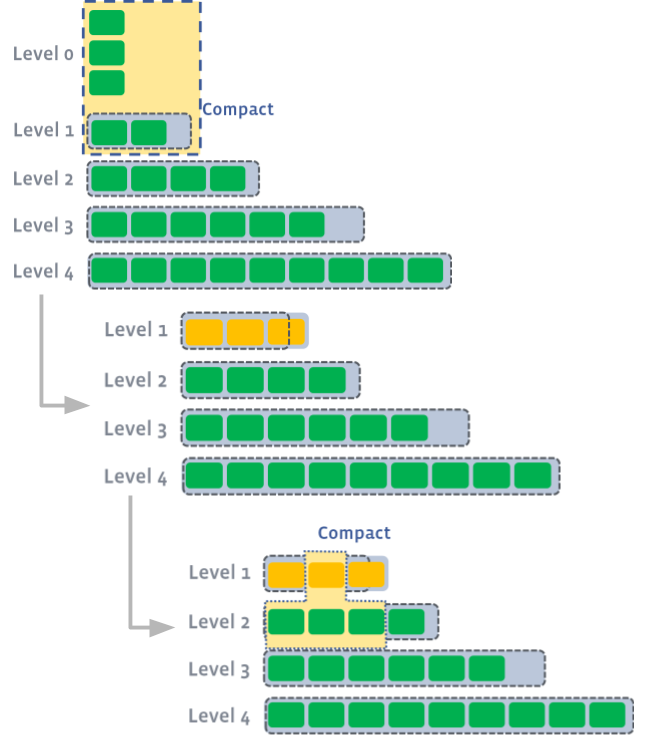
\includegraphics[width=0.5\textwidth]{level_compaction}
  \caption{SS-tables from initial levels are compacted into the next~\cite{rocksdb-compaction}.}
\end{figure}

In RocksDB, compactions are triggered when the previous \textit{level} reaches a
certain size. Referred to as \textit{leveled compaction}, this was one of the
original contributions of LevelDB\@. As described in~\cite{rocksdb-compaction},
this is usually initiated when the amount of SS-tables at the first level, level
0, goes beyond a certain amount. This in turn might cause the next level to go
beyond its size limit, resulting in a compaction to the next level again, and so
on. Unlike LevelDB, RocksDB also supports doing compactions in parallel, as long
as there are enough available background threads to do so.

\subsection{Bloom filters}\label{sec:bloom}
Iterating through every SS-table available to find a single key is inefficient.
Instead, we would like to ask the question ``can this key possibly exist here?''
for each of the SS-tables we go through, and only operate on the ones where the
answer is ``yes''. With a regular hash based data structure this would be quite
costly in terms of space, as we would need to maintain such a structure for
every SS-table in our database. Instead, RocksDB, and many other systems like
it, rely on a probabilistic data structure known as a bloom filter~\cite{bloom}
to do so.

Instead of knowing with 100\% certainty whether a key exists in a set, a bloom
filter would let us know if that key \textit{might possibly} be in the set, or
if it is \textit{definitely} not. The third option, of possibly \textit{not}
being in the set is impossible. The positive trade-off here is that it uses
significantly less space, opening the possibility of using it for every SS-table
in the system.

\subsection{Iteration}
One of the essential features of RocksDB compared to other key-value stores is
that its data is \textit{sorted}, and that it can be queried as such through
\textit{iterators}. This opens for a wide variety of possibilities that would
not have been feasible with a regular key-value store, such as range queries.
RocksDB supports iterating both forwards and backwards.

Similar to with reads, performing a fully ordered scan in an LSM-tree based
storage engine is far from optimal: every tree-structure, or SS-table in
RocksDB, needs to be considered, and as key ranges may overlap between different
files, sorted.

A lot of applications do not rely on completely random scans of keys however,
and only need support for ordered queries within a specific \textit{key prefix}.
Developers instruct RocksDB on how to retrieve a specific prefix from each key,
which RocksDB then internally uses to organize the data in such a manner that
iterating through keys within a \textit{specific prefix} is efficient: either by
storing bloom filters for each prefix, or by managing a hash based index
structure based on the prefix.

% TODO: might show an example to better explain prefix stuff here, or save it
% for implementation.

\subsection{Column Families}

RocksDB supports the equivalent of tables from a traditional database through
\textit{column
families}\furl{https://github.com/facebook/rocksdb/wiki/Column-Families}.
Separate column families share the same write-ahead log but have their own
MemTables and SS-tables. Maintaining the same WAL makes it possible to
atomically write across multiple column families, while keeping independent
LSM-tree components open for the possibility of configuring different column
families separately---an important difference from tables in SQL databases.

Column family support was not added until version 3.0 of RocksDB.\@ To maintain
backwards compatibility, the default API methods operate on the same column
family, ``default'', with separate methods taking in an additional column family
argument.

\subsection{RocksDB from Rust}
While RocksDB is written in C++ it provides a separate API through its
C-bindings, which are used to call into it from a variety of different
languages\furl{https://github.com/facebook/rocksdb/blob/master/LANGUAGE-BINDINGS.md}.

% TODO: ref to appendix?
% TODO: ref to ffi section
This thesis makes use of a modified version of
\textbf{rust-rocksdb}\furl{https://github.com/spacejam/rust-rocksdb}, which exposes a Rust-friendly
API that eventually calls into the C-bindings.

\begin{listing}[H]\label{lst:rocksdb-rust}
  \begin{minted}[frame=lines]{rust}
let db = DB::open_default("db_path").unwrap();

let key = b"key";
let value = b"value";
db.put(key, value).unwrap();

match db.get(key) {
  Ok(v) => assert_eq!(*v.unwrap(), value),
  Err(e) => panic!("failed reading from rocksdb: {}", e),
}
  \end{minted}

  \caption{Simple example usage of rust-rocksdb}
\end{listing}
